\documentclass[12pt]{article}

\usepackage{graphicx}
\usepackage{amsmath}
\usepackage{amssymb}
\usepackage{natbib}
\usepackage{amsfonts}
\usepackage{multicol}
\usepackage{float}
\usepackage{oldgerm}
\usepackage{bm}
\usepackage{mathtools}
\usepackage{wrapfig}
\usepackage{fancyhdr}
\usepackage[export]{adjustbox}
\usepackage{xcolor}

\pagestyle{empty}

\newcommand{\Avec}{\mathbf A}
\newcommand{\Bvec}{\mathbf B}
\newcommand{\Dvec}{\mathbf D}
\newcommand{\Evec}{\mathbf E}
\newcommand{\Fvec}{\mathbf F}
\newcommand{\Jvec}{\mathbf J}
\newcommand{\Lvec}{\mathbf L}
\newcommand{\Mvec}{\mathbf M}
\newcommand{\Pvec}{\mathbf P}
\newcommand{\Svec}{\mathbf S}
\newcommand{\avec}{\mathbf a}
\newcommand{\bvec}{\mathbf b}
\newcommand{\dvec}{\mathbf d}
\newcommand{\evec}{\mathbf e}
\newcommand{\fvec}{\mathbf f}
\newcommand{\jvec}{\mathbf j}
\newcommand{\kvec}{\mathbf k}
\newcommand{\nvec}{\mathbf n}
\newcommand{\pvec}{\mathbf p}
\newcommand{\rvec}{\mathbf r}
\newcommand{\svec}{\mathbf s}
\newcommand{\vvec}{\mathbf v}
\newcommand{\xvec}{\mathbf x}
\newcommand{\yvec}{\mathbf y}
\newcommand{\zvec}{\mathbf z}
\newcommand{\nablav}{\boldsymbol{\nabla}}
\newcommand{\nablavector}{\vec \nabla}
\newcommand{\alphavec}{\boldsymbol{\alpha}}
\newcommand{\phivec}{\boldsymbol{\phi}}
\newcommand{\thetavec}{\boldsymbol{\theta}}
\newcommand{\omegavec}{\boldsymbol{\omega}}
\newcommand{\tauvec}{\boldsymbol{\tau}}
\newcommand{\ezero}{\varepsilon_{0}}
\newcommand{\mzero}{\mu_{0}}
\newcommand{\mubold}{\boldsymbol{\mu}}
\newcommand{\uniti}{\hat{\boldsymbol{\imath}}}
\newcommand{\unitj}{\hat{\boldsymbol{\jmath}}}
\newcommand{\unitk}{\hat{\boldsymbol{\mathit{k}}}}
\newcommand{\unitn}{\hat{\mathbf n}}
\newcommand{\unitr}{\hat{\mathbf r}}
\newcommand{\unitphi}{\hat{\boldsymbol{\phi}}}
\newcommand{\unittheta}{\hat{\boldsymbol{\theta}}}

\newcommand{\bit}{\begin{itemize}}
\newcommand{\eit}{\end{itemize}}

\setlength{\headsep}{0.5cm}
\setlength{\oddsidemargin}{-0.5cm}
\setlength{\textwidth}{16.5cm}
\setlength{\textheight}{24cm}
\voffset = -2cm

\pagestyle{fancy}
\fancyhf{}
\rfoot{
\includegraphics[width=1.0in]{cnm.png}}
\lfoot{Homework 9}
\begin{document}

%{\bf \underline{STUDENT NAME}:} 
%\vspace{1cm}

\begin{center}
\hfil
%\begin{wrapfigure}{l}{0.5in} 
%    
\includegraphics[width=0.5in]{cnm.png}
%\end{wrapfigure}
{\large\bf {ENGR 2910-101: Circuit Analysis}}
\hfill Instructor: Leo Silbert \\
Homework 9: 11/03/21 \hfill Due: 11/10/21\\
\hrulefill\\
\end{center}

%{\em Show all your working to ensure you obtain full points. Partial
%  credit will be given for correct algebraic steps if you fail to
%  obtain the correct final answer.}\\

%\newpage


\noindent
{\bf Question 1} [10]

\begin{figure}[h!]
     \centering
\vspace{-0.1in}
     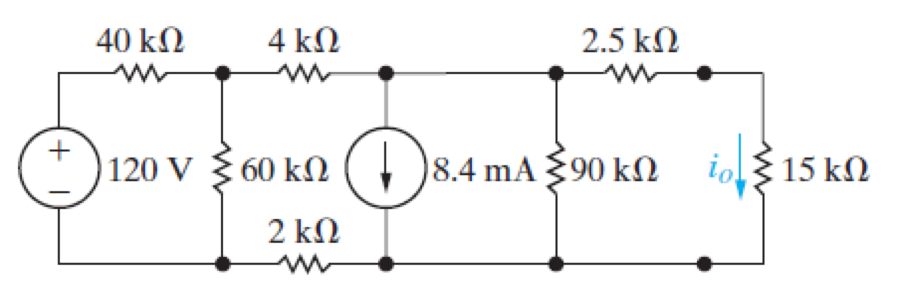
\includegraphics[clip,width=0.7\textwidth]{Fig4-60.png}
\vspace{-0.15in}
\end{figure}
\bit

\item[(i)]

Using several source transformations find the value of the current flowing through the $15~k\Omega$ resistor. [Hint: start on the left side of the circuit and work your way right.]

\item[(ii)]

Now that you know this current, work backwards through the original circuit and calculate the following: the voltage drop across the $90~k\Omega$ and the current flowing through that branch; the current flowing through the $4~k\Omega$ resistor, the voltage drop across the $60~k\Omega$ resistor; and the current flowing in the left-hand part of the circuit. 

\eit 

\newpage
\noindent
{\bf Question 2} [10]

Find the Th\'evenin equivalent for the following circuit. [Hint: start off by making a source transformation then apply the mesh-current method.]
\begin{figure}[h!]
     \centering
\vspace{-0.1in}
     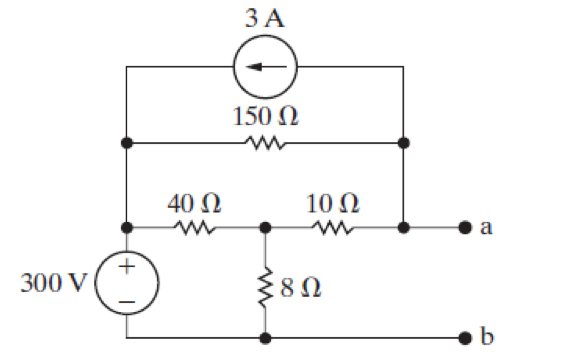
\includegraphics[clip,width=0.7\textwidth]{Fig4-67.png}
\vspace{-0.15in}
\end{figure}

\newpage
\noindent
{\bf Question 3} [10]

Find the Norton equivalent for the following circuit. [Hint: apply the node-voltage and mesh-current methods.]
\begin{figure}[h!]
  \centering 
  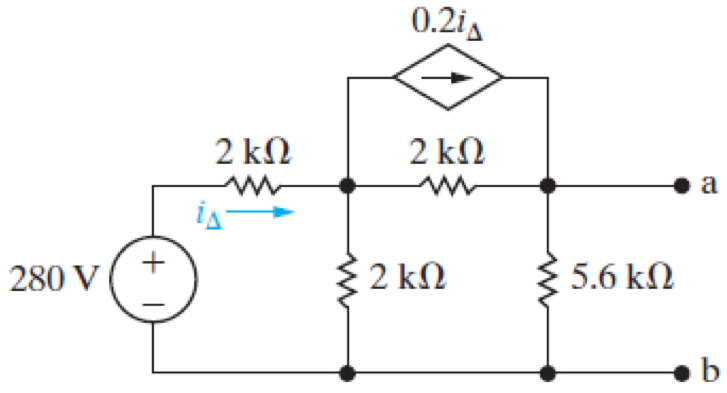
\includegraphics[clip,width=0.5\textwidth]{Fig4-75.png}
\end{figure}

\newpage
\noindent
{\bf Question 4} [10]

Use the test source method to find the Th\'evenin resistance. [Hint: use the node-voltage method.]
\begin{figure}[h!]
  \centering 
  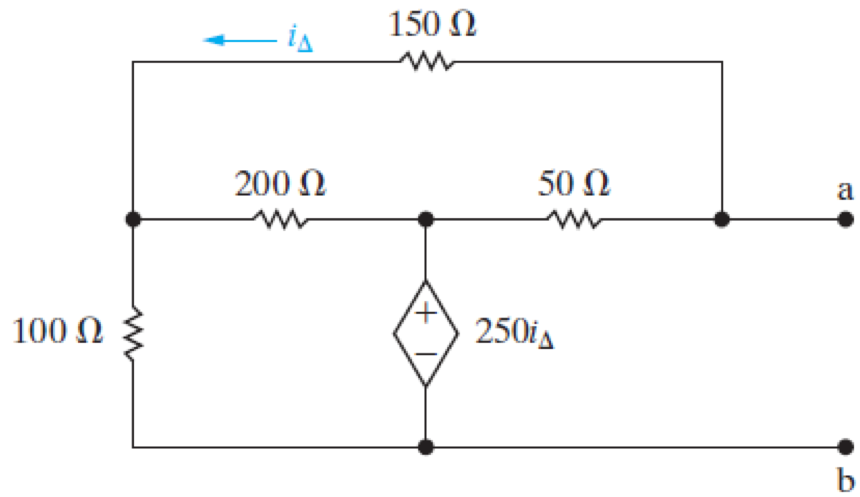
\includegraphics[clip,width=0.6\textwidth]{Fig4-79.png}
\end{figure}

\newpage
%\vspace{0.1in}
\noindent
{\bf Question 5} [10]

Use the principle of superposition to find the voltage $v_{o}$. [Hint: when you analyze the current source, apply the node voltage method choosing the reference node as the node below the $40~\Omega$ resistor.]
\begin{figure}[h!]
\centering 
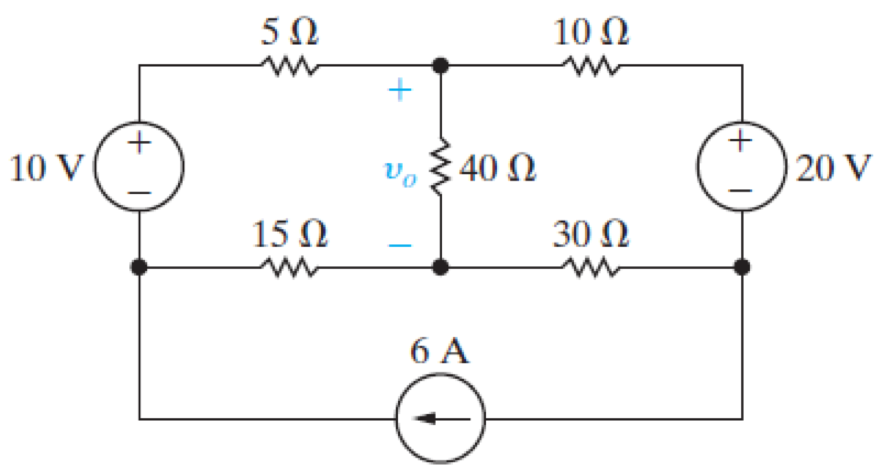
\includegraphics[clip,width=0.6\textwidth]{Fig4-94.png}
\end{figure}


\end{document}
